\chapter{Hall sensor test} %\label{put a label here and uncomment}
\textbf{Name: Group 510}\\
\textbf{Date: 06/10 - 2015}

\section*{Purpose}
The belt vehicle is equipped with two hall sensors, one mounted on each driving wheel. The sensors have no visible markings, so a data sheet can not be found. This test helps determining the pinout of the sensors, and to test if they work.
\\

\section*{Setup}
The test setup can be seen in \figref{hallTest}
\begin{figure}[H]
	\centering
	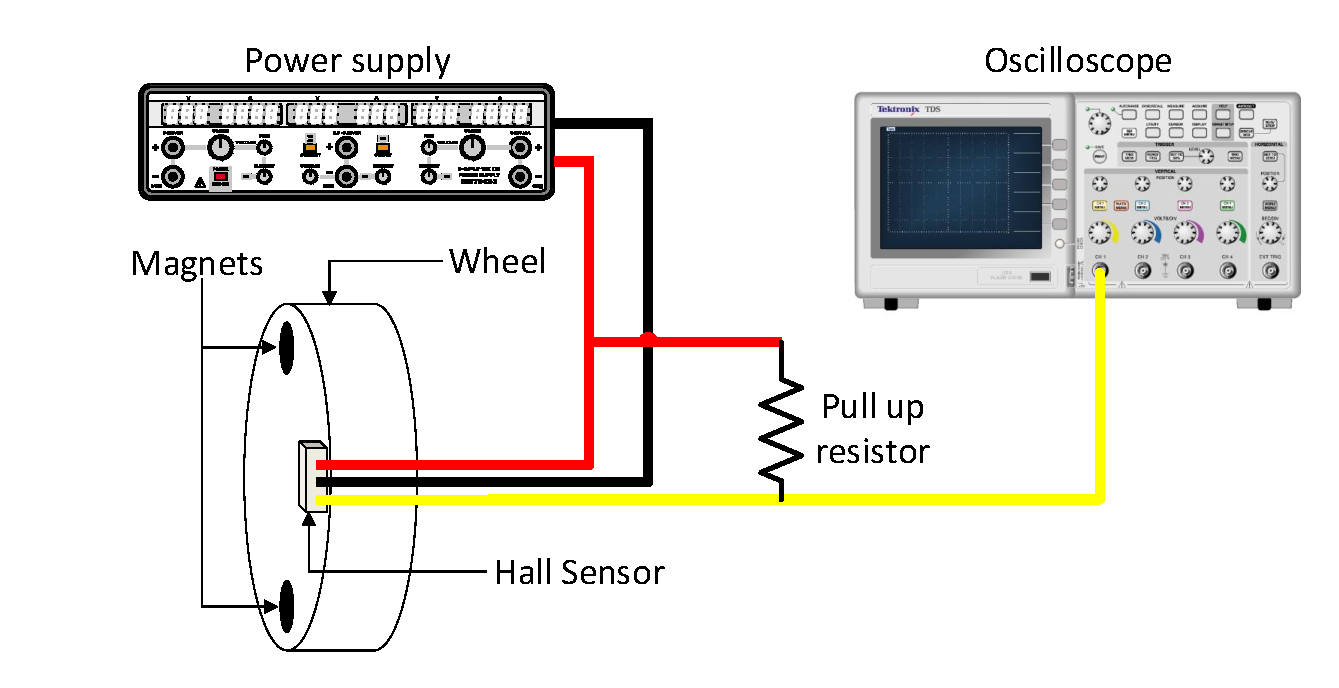
\includegraphics[scale=.6]{figures/hall-test-setup.pdf}
	\flushleft
	\caption{Test setup for hall sensors}
	\label{hallTest}
\end{figure}\vspace{-5mm}

\section*{List of Equipment}
\begin{table}[H]
\begin{tabular}{|l|l|p{4cm}|}
\hline%-------------------------------------------------------------------
  \textbf{Instrument}           &  \textbf{AAU-no.}  &  \textbf{Type}    \\
\hline%-------------------------------------------------------------------
  Oscilloscope                  &  64588             &  Tektronix TDS2004B  \\
\hline%-------------------------------------------------------------------
  Power supply							&  60771                  &   Hameg HM7042-3  \\
\hline%-------------------------------------------------------------------

\end{tabular}\\
\end{table}

\section*{Procedure}

\begin{enumerate}
\item write each step as done after setup - if there are different configurations of setup remember to include these.
\end{enumerate}

\section*{Results}

Example of results:
\begin{table}[H]
\begin{tabular}{|l|l|l|l|}

\hline%------------------------------------------------------------------------------------------------------
           & \textbf{Expected Result}   & \textbf{Result} \\
\hline%------------------------------------------------------------------------------------------------------
  \textit{Frequency}           &  49.5 - 50.5 $Hz$ &  50 $Hz$  \\
\hline%------------------------------------------------------------------------------------------------------
\textit{Ammplitude}                     &   3.1 - 3.4 $V$            &    3.3 $V$          \\
\hline%------------------------------------------------------------------------------------------------------
 \textit{Pulse Width: Min}     &    5 \% (1 $ms$)          &     1  $ms$   \\
\hline%------------------------------------------------------------------------------------------------------
\textit{Pulse Width: Med}      &      7.5 \% (1.5 $ms$)           & 1.5 $ms$            \\
\hline%------------------------------------------------------------------------------------------------------
  \textit{Pulse Width: Max}   &    10 \% (2 $ms$)             &  2 $ms$         \\
\hline%------------------------------------------------------------------------------------------------------

\end{tabular}
\end{table}